\documentclass[12 pt]{report}
\usepackage{fullpage, amssymb, amsmath, graphicx, caption, subcaption}

% Title Page
\title{Using Convex Optimization to Control Linear Systems with Disturbances}
\author{Oladapo Afolabi, Sarah Seko, Alek Williams}
\date{December 4, 2015}

\begin{document}
\maketitle

\begin{abstract}
\end{abstract}

\section{Introduction}
This report concerns the application of convex optimization to control linear systems subject to disturbances. In discrete time, the system dynamics are of the form $$ x_{t+1} = Ax_t + Bu_t + B_w w_t $$ where $x_t \in \mathbb{R}^n$ is the state vector, $u_t \in \mathbb{R}^m$ is the input vector, $w_t \in \mathbb{R}^p$ is a vector of disturbances, and $A$, $B$, and $B_w$ are real matrices of appropriate dimension. Three techniques were studied: affine recourse, tube 

\section{Model Predictive Control}

Model Predictive Control (MPC) is a suboptimal control scheme for approximating the solution of an optimal control problem using a receding horizon approach \cite{MPCbook}. An optimal control problem uses a model of the plant to predict its behavior and solve for the optimal control policy. Suppose that the system of interest evolves according to the discrete time dynamics $x_{t+1} = f(x_t, u_t)$ and the initial state of the system, $\bar{x}_0$, is known. The system is restricted such that the state must be contained in the set $\mathcal{X}$ at all time steps. Additionally, the input to the system is also limited to be in the set $\mathcal{U}$. A stage cost, $\ell (x_t, u_t)$ is defined as a function of the current state and input. We would like to find the optimal control policy, $\psi(\cdot)$, which takes as its argument the current state of the system and returns the input, with respect to the stage cost while respecting the state and input constraints. The optimal control problem is given below \cite{schildbach14}.

\begin{equation*}
\begin{aligned}
& \min_{\psi(\cdot)} & & \sum_{t = 0}^{T-1} \ell (x_t, u_t) \\
& \text{subject to} & & x_0 = \bar{x}_0 \\
& & & x_{t+1} = f(x_t, u_t); ~ \forall t = 0, \dots, T-1 \\
& & & x_t \in \mathcal{X}; ~ \forall t = 1, \dots, T \\
& & & u_t \in \mathcal{U}; ~ \forall t = 0, \dots, T-1 \\
& & & u_t = \psi (x_t); ~ \forall t = 0, \dots, T-1
\end{aligned}
\end{equation*}

The system dynamics can be substituted to eliminate the predicted state of the system so the only optimization variable is the control policy. The optimal control problem is in general intractable because it is an infinite dimensional optimization problem over the set of all functions. The time period of interest may also be prohibitively long, even infinite. In order to solve the problem, the objective function is minimized over the open-loop inputs instead of all control policies. A receding horizon approach is also adopted, where the problem is solved for a shorter horizon $N$, called the prediction horizon, instead of the whole horizon $T$ before shifting the prediction horizon and solving the problem again. To close the loop with the plant, the measured state at each time step is used as the initial condition of the optimization problem, which is given below.

\begin{equation*}
\begin{aligned}
& \min_{u_{0|t}, \dots, u_{N-1|t}} & & \sum_{i = 0}^{N-1} \ell (x_{i|t}, u_{i|t}) \\
& \text{subject to} & & x_{0|t} = x_t \\
& & & x_{i+l|t} = f(x_{i|t}, u_{i|t}); ~ \forall i = 0, \dots, N-1 \\
& & & x_{i|t} \in \mathcal{X}; ~ \forall i = 1, \dots, N \\
& & & u_{i|t} \in \mathcal{U}; ~ \forall i = 0, \dots, N-1 \\
\end{aligned}
\end{equation*}

The notation $\cdot_{i|t}$ is used to indicate a predicted quantity that is $i$ steps into the future given that the current time step is $t$. Again, the system dynamics can be substituted to eliminate the state variables, leaving the open-loop inputs as the only optimization variables. If the system evolves with linear dynamics then the equality constraints are all affine. If the sets $\mathcal{X}$ and $\mathcal{U}$ are convex and the stage cost is a jointly convex function of the state and input then the problem is convex.

Now consider the case where the system dynamics are linear but subject to stochastic disturbances of known distribution. $$ x_{t+1} = Ax_t + Bu_t + w_t $$ The predicted states are now random variables making it meaningless to optimize over the sum of stage costs or enforce constraints. Instead, the stage costs must be replaced by their expected values. This can also be used on the constraints, specifying that the expected value of the states must be contained in $\mathcal{X}$. Alternatively, the probability that the state lies within $\mathcal{X}$ can be constrained to be greater $1 - \epsilon$, where $\epsilon$ is a small number, called the violation level. The stochastic problem is shown below with these so-called chance constraints.

\begin{equation*}
\begin{aligned}
& \min_{u_{0|t}, \dots, u_{N-1|t}} & & \sum_{i = 0}^{N-1} \mathbb{E} \left[ \ell (x_{i|t}, u_{i|t}) \right] \\
& \text{subject to} & & x_{0|t} = x_t \\
& & & x_{i+l|t} = Ax_{i|t} + Bu_{i|t} + w_{t+i}; ~ \forall i = 0, \dots, N-1 \\
& & & \mathrm{Pr} \left\{ x_{i|t} \in \mathcal{X}  \right\} \geq 1 - \epsilon; ~ \forall i = 1, \dots, N \\
& & & u_{i|t} \in \mathcal{U}; ~ \forall i = 0, \dots, N-1 \\
\end{aligned}
\end{equation*}

The stochastic problem is in general nonconvex and intractable but there exist computationally feasible convex formulations to approximate the problem, two of which were selected to be studied and are discussed in this report.

\section{Scenario MPC}

In Scenario MPC (SCMPC), the stochastic problem is approximated by a deterministic one by taking samples of the disturbance \cite{schildbach14}. Together with the predicted inputs, a set of samples for each step in the prediction horizon $w_t^{(k)} = \{w_{0|t}^{(k)}, \dots, w_{N-1|t}^{(k)} \} $, called a scenario, generates a state trajectory. The notation $\cdot_{i|t}$ is again used to indicate that these are predicted values and not the realizations of the disturbance that will occur in the actual system. The expected value in the cost function of the stochastic problem is approximated by the average of the cost functions for each trajectory, the same as optimizing over the sum of the cost functions. The predicted input sequence, $u_{0|t}, \dots, u_{N-1|t}$, is required to be feasible with respect to the state constraints on each trajectory created by the scenarios. The SCMPC problem, which is convex under the same conditions given for the general MPC problem, is given below.

\begin{equation*}
\begin{aligned}
& \min_{u_{0|t}, \dots, u_{N-1|t}} & & \sum_{k = 1}^{K} \sum_{i = 0}^{N-1} \ell (x_{i|t}^{(k)}, u_{i|t}) \\
& \text{subject to} & & x_{0|t}^{(k)} = x_t; ~ \forall k = 1,\dots,K \\
& & & x_{i+l|t}^{(k)} = Ax_{i|t}^{(k)} + Bu_{i|t} + w_{i|t}^{(k)}; ~ \forall i = 0, \dots, N-1, ~k = 1,\dots,K \\
& & & x_{i|t}^{(k)} \in \mathcal{X}; ~ \forall i = 1, \dots, N, ~k = 1,\dots,K \\
& & & u_{i|t} \in \mathcal{U}; ~ \forall i = 0, \dots, N-1 \\
\end{aligned}
\end{equation*}

The number of sampled scenarios, $K$, is called the sample complexity and must be chosen so that the chance constraints are satisfied. A sample complexity that guarantees satisfaction of the chance constraints is called admissible. Intuitively, as more scenarios are used, the violation probability of the system will decrease because the solution of the SCMPC problem will be robust with respect to more realizations of the disturbance. The computational complexity of the problem, however, grows with the number of scenarios. Although the number of decision variables remains the same, the number of constraints grows linearly with the number of scenarios. The goal is then to find the smallest admissible $K$, which would satisfy the chance constraints with the minimal possible computation.

The required sample complexity is related to a property of the chance constraint called the support rank. The support rank is a property of an individual chance constraint so each chance constraint can be considered separately and for possibly different desired violation levels. Let $\mathcal{L}_i$ denote the unconstrained subspace of the $i$-th step constraint, $i \in \{0,\dots,N-1\}$, which is the largest subspace of the search space $\mathbb{R}^{Nm}$ that is unconstrained by all scenarios, almost surely. Then the support rank, $\rho_i$ is the co-dimension of $\mathcal{L}_i$. $$ \rho_i := Nm - \dim \mathcal{L}_i$$
Consider, for example, a single linear inequality constraint on the predicted state, $ g^\top x_{i|t} \leq h$, where $h \in \mathbb{R}$. Substituting the linear stochastic dynamics of the system for the predicted state creates the inequality constraint on the decision variables, the open-loop inputs.
\begin{displaymath}
\begin{bmatrix}
\tilde{g}_{0}^\top & \dots & \tilde{g}_{i-1}^\top & 0 & \dots & 0 
\end{bmatrix}
\begin{bmatrix}
u_{0|t} \\ \vdots \\ u_{N-1|t}
\end{bmatrix} + \tilde{h} \leq h
\end{displaymath}
The vectors $\tilde{g}_i$ are deterministic functions of $g$ and the system matrices $A$ and $B$. The zeros are included to show that the predicted state $x_{i|t}$ is only a function of the open-loop inputs up to time $i-1$. The scalar $\tilde{h}$ is a random variable that is a function of the stochastic disturbances. Therefore, no matter the values of the scenarios generated, the hyperplane created by the constraint will always be parallel to the hyperplane in the deterministic case. Any subspace that is parallel to these hyperplanes will be unconstrained by the constraints and so the support rank of the linear inequality constraint is $\rho_i = 1$ \cite{schildbach13}.
The first step violation probability, $V_t|x_t$ is the probability that the first predicted state, $x_{1|t}$ will fall outside of the set $\mathcal{X}$ given that initial state $x_{0|t} = x|t$. $$V_t|x_t = \mathrm{P}\left( Ax_{0|t} + Bu_{0|t} + w_{t} | x_{0|t} = x_t \right) $$
The expected value of the first step violation probability can be bounded above by a function of the support rank of the first time step state constraint and the sample complexity. $$ \mathbb{E} \left[ V_t|x_t \right] \leq \frac{\rho_1}{K+1} $$
The desired sample complexity is then given by the smallest $K$ that satisfies $ \frac{\rho_1}{K+1} \leq \epsilon $ \cite{schildbach14}.

\section{Tube Scalings}

A scaling random variable $\alpha_k$ is defined such that the disturbance $w_k$ lies in an ellipsoid parameterized by the random variable. $$w_k \in \mathcal{E}(W, \alpha_k) := \{w: w^\top Ww \leq \alpha\}$$ The random variable $\alpha_k$ is assumed to be bounded by $\bar{\alpha}$ and its cumulative distribution function, $F_\alpha$, is known in closed form or can be numerically integrated. For example, if each component of $w_k$ is an identically and independently distributed truncated Gaussian random variable and $W$ is the identity matrix, then $\alpha_k$ has a truncated $\chi^2$ distribution. 

Scaling random variables $\beta_i$ are also defined such that the predicted deviations lie in ellipsoids parameterized by $\beta_i$. $$ e_{i|k} \in \mathcal{E}(V, \beta_i) := \{e : e^\top Ve \leq \beta_i\}  $$ So that the predicted deviations that are in the bounding ellipsoid at one time step are guaranteed to lie within the next bounding ellipsoid at the next time step, the scaling variables evolve according to $ \beta_{i+1} = \lambda \beta_i + \alpha_i $. For $\lambda \in (0,1)$, this implies that $\beta_{i+1}$ is bounded above by $\bar{\beta}_{i+1} = \lambda\bar{\beta}_i + \bar{\alpha} $ and the bounds themselves are bound by $\bar{\beta}_i \leq \bar{\beta} = \max \{ \bar{\beta}_0, \frac{\lambda}{1 - \lambda} \bar{\alpha}\}$. 

Because $\beta_{i+1}$ is the sum of two random variables, its cumulative distribution function $F_{\beta_{i+1}}$ can be found by taking the scaled convolution of the cumulative distribution function of the previous scaling variable and the density function of $\alpha$. $$ F_{\beta_{i+1}}(x) = \lambda \int_{-\infty}^{\infty} F_{\beta_i}(y)f_\alpha (x-\lambda y)dy $$ The random variable $\beta_i$ is nonnegative so $F_{\beta_i}$ only has support on $[0, \infty)$. The random variable $\alpha_i$ is nonnegative and bounded so $f_\alpha$ only has support on $[0, \alpha]$. Thus the limits of the convolution integral are finite and given in the following equation. $$ F_{\beta_{i+1}}(x) = \lambda \int_{0}^{\bar{\beta}/\lambda} F_{\beta_i}(y)f_\alpha (x-\lambda y)dy $$

A numerical integration scheme was employed to calculate approximations of the distributions of $\beta_i$, which are denoted by $\pi_i$. These vectors are the approximation of the cumulative distribution functions $F_{\beta_i}$ evaluated at $\rho+1$ equally spaced points between $0$ and $\bar{\beta}$. Let $x$ be the vector of evaluation points for $\pi_i$, meaning that $\pi_{i,j} \approx F_{\beta_i}(x_j)$. Let $h = x_{j+1} - x{j}$ be the distance between the evaluation points and $\omega$ the number of segments of length $h$ between $\bar{\beta}$ and $\bar{\beta}/\lambda$. Using the trapezoid rule for integration, a matrix P can be defined such that the next distribution can be found by  
$$\pi_{i+1} = P \begin{bmatrix}
\pi_i \\ \mathbf{1}_\omega
\end{bmatrix} $$ where $\mathbf{1}_\omega$ is a vector of ones with length $\omega$.

\begin{displaymath}
	P = \frac{h}{2}\begin{bmatrix}
		f_\alpha(x_0 - \lambda x_0) & 2f_\alpha(x_0 - \lambda x_1) & \dots & 2f_\alpha(x_0 - \lambda x_{\rho + \omega - 1}) & f_\alpha(x_0 - \lambda x_{\rho + \omega}) \\
		f_\alpha(x_1 - \lambda x_0) & 2f_\alpha(x_1 - \lambda x_1) & \dots & 2f_\alpha(x_1 - \lambda x_{\rho + \omega - 1}) & f_\alpha(x_1 - \lambda x_{\rho + \omega}) \\
		\vdots & \vdots & & \vdots & \vdots \\
		f_\alpha(x_\rho - \lambda x_0) & 2f_\alpha(x_\rho - \lambda x_1) & \dots & 2f_\alpha(x_\rho - \lambda x_{\rho + \omega - 1}) & f_\alpha(x_\rho - \lambda x_{\rho + \omega}) \\
	\end{bmatrix}
\end{displaymath}

 First, $\beta_0$ was assumed to be deterministically 0 so $\pi_0 = \mathbf{1}_{\rho + 1}$. The subsequent approximations of $F_{\beta_i}$ can be found by $\pi_i = P^i \pi_0$. However, the approximated distributions were not smooth because of the numerical integration and they did not satisfy the properties of a cumulative distribution, specifically that $\pi_i$ should be a nondecreasing sequence of numbers. To create better approximations of $F_{\beta_i}$, the following convex optimization problem was solved.
 
\begin{equation*}
\begin{aligned}
& \min_{\hat{\pi}_i} & & \|\hat{\pi}_i - \pi_i \|_2^2 + \mu \sum_{j = 0}^{\rho} (\hat{\pi}_{i,j+1} - \hat{\pi}_{i,j})^2\\
& \text{subject to} & & 0 \leq \hat{\pi}_{i,j} \leq 1; ~ \forall j = 0, \dots, \rho \\
& & & \hat{\pi}_{i,j} \leq \hat{\pi}_{i,j+1}; ~ \forall j = 0, \dots, \rho -1 \\
\end{aligned}
\end{equation*}

In the problem, $\pi_i$ is the one-step advance distribution obtained by multiplying the previous distribution with $P$. The decision variables $\hat{\pi}_i$ are a smoothed approximation of the distribution that satisfies the properties of a cumulative distribution function, which is enforced by the constraints of the problem. The parameter $\mu$ is used to balance the weight between approximating the unsmoothed distribution and the smoothness of new distribution. The value $\mu = 100$ was found to give good results. For the remainder of this report, the notation $\pi_i$ is used to refer to the smoothed distributions obtained by solving the above problem. When calculating a multiply step advance distribution, the distributions were smoothed in between each multiplication by $P$.

For notation convenience, the following functions are defined.
\begin{align*}
\mathrm{ind}(\pi_i,p) &= \min\{j:\pi_{i,j} \geq p\} \\
b(\pi_i,p) &= x_j, ~j = \mathrm{ind}(\pi_i, p)
\end{align*}
The function $\mathrm{ind}(\pi_i,p)$ is the index of the first element of the distribution $\pi_i$ to exceed the probability level $p$. The function $b(\pi_i,p)$ is the value of the element in input vector $x$ that corresponds to $\mathrm{ind}(\pi_i,p)$. This means that $F_{\beta_i}(b(\pi_i,p)) \approx p$ or alternatively  $\mathrm{Pr} \{\beta_i \geq b(\pi_i,p) \} \approx p$. It follows from these definitions that $e_{k+i} \in \mathcal{E}(V,b(\pi_i,p))$ with probability $p$.

\section{Recursive Feasibility}
To ensure recursive feasibility of the tube MPC problem, the constraints are tightened further based on the upper bound on $\beta_i$. Let $\pi_{i|j}, j < i$ be the approximated distribution of $\beta_i$ assuming that the value of $\beta_j$ is equal to its upper bound according to the distribution $\pi_{j|0}$. Using the previous notation, $\pi_i = \pi_{i|0}$ because $\beta_0$ is deterministic. Define $\pi_{i|i}$ to be the distribution such that elements before $\mathrm{ind}(\pi_i,1)$ are all zero and the remaining elements are ones. Then the same P matrix can be used to find $\pi_{i|j}$.
$$ \pi_{i|j} = P^{i-j} \begin{bmatrix}
\pi_{j|j} \\ \mathbf{1}_\omega
\end{bmatrix} $$
Define $\bar{b}_i$ to be the largest scaling over the different distributions generated by starting from the upper bound of $\beta_j$ based on $\pi_j$ for $j = 1, \dots, i-1$. $$ \bar{b}_i(q) = \max \{ b(\pi_{i|0},q), \dots, b(\pi_{i|i-1},q) \} $$ Using these tube scalings instead of those generated by starting at the distribution of $\beta_0$ will guarantee recursive feasibility of the tube MPC problem.

\section{Example 2 (from Schildbach et al. 2014)}

The dynamic system used in this example was adapted from Schildbach et al. (2014). The stochastic dynamics are given below. 
\begin{equation*}
x_{t+1} = \begin{bmatrix}
0.7 & -0.2 \\ -0.3 & 0.9
\end{bmatrix} x_t + 
\begin{bmatrix}
1 & 0 \\ 0 & 1
\end{bmatrix} u_t + 
\begin{bmatrix}
w_t^{(1)} \\ w_t^{(2)}
\end{bmatrix}
\end{equation*}
The disturbances $w_t^{(1)}$ and $w_t^{(2)}$ are independent and normally distributed with mean 0 and variance 0.1. The state is constrained such that $x_t^{(1)},  x_t^{(2)} \geq 1$ and the input is constrained such that $|u_t^{(1)}|, |u_t^{(2)}| \leq 5$. The goal is to drive the state to the origin using minimal control effort so the cost function chosen was the squared norm of the state and the input. The prediction horizon was set to 6 time steps and the initial condition was $x_0 = [1~ 1]^\top$.

The two state constraints were considered individually and the desired violation level was set to $\epsilon = 10\%$ for each. The two chance constraints used for this problem are given below.
\begin{align*}
\mathrm{Pr} (x_t^{(1)} \geq 1) \geq 1 - \epsilon = 0.9 \\
\mathrm{Pr} (x_t^{(2)} \geq 1) \geq 1 - \epsilon = 0.9
\end{align*}
In each case, the chance constraints are single linear inequalities so they both have a support rank of $\rho = 1$. Therefore, the minimal sample complexities required to achieve the desired violation levels are $K_1 = K_2 = 9$.

The system was simulated for 3000 closed loop time steps, as shown in Figure \ref{fig:SCMPC_3000}. The number of constraint violations was 296 for $x_1$ and 300 for $x_2$ giving empirical violation levels of 9.87\% and 10\%, respectively.

\begin{figure}
	\centering
	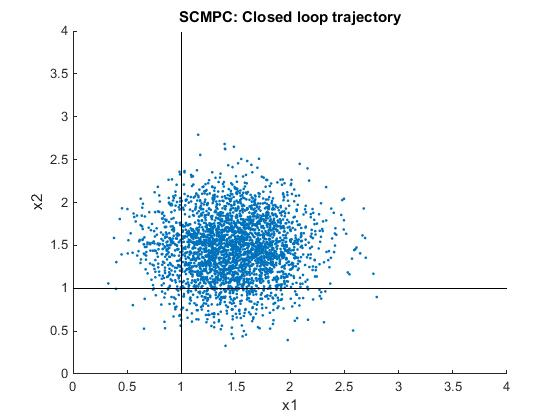
\includegraphics[width=3.5in]{SCMPC_3000.jpg}
	\caption{The closed loop system trajectory using the scenario MPC controller is plotted with blue dots for 3000 closed loop time steps. The state constraints are plotted as solid black lines.}
	\label{fig:SCMPC_3000}
\end{figure}


\section{Example 1 (from Cannon et al. 2010)}

In this example, there is only a single linear inequality constraint on the state. The constraint has a support rank $\rho = 1$ so the necessary sample complexity to achieve the specified violation level of $\epsilon = 0.2$ is $K = 4$. The simulation was run for 200 systems for 6 closed loop time steps, each time using CVX to solve the scenario MPC problem with 4 scenarios. The system trajectories are shown in Figure \ref{fig:SCMPC_200x6}. The empirical constraint violations were 21\% for $t = 1$ and 0\% for all other time steps.

\begin{figure}
	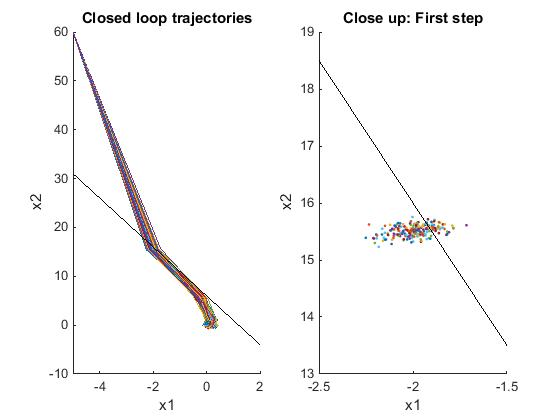
\includegraphics[width=\linewidth]{SCMPC_200x6.jpg}
	\caption{The closed loop system trajectory using the scenario MPC controller is plotted on the left for 200 simulated systems, each for 6 time steps. A close up of the state after one time step, which has some constraint violations, is shown on the right. The state constraint is plotted as a solid black line.}
	\label{fig:SCMPC_200x6}
\end{figure}

\section{Example: Cart-Pendulum system}

\begin{figure}
	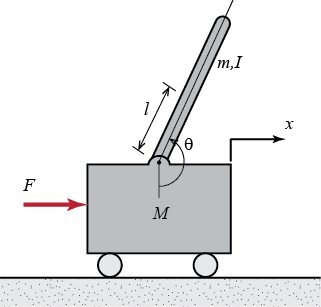
\includegraphics[width=\linewidth]{cart-pendulum.jpg}
	\caption{An image showing the coordinate systems of the cart and pendulum system.}
	\label{fig:cart-pendulum}
\end{figure}

The three control techniques were then applied to the system of a pendulum hanging from a cart, shown in Figure \ref{fig:cart-pendulum}. The system was adapted from \cite{pendulum} so that rotational damping was included and the system was linearized about the stable equilbrium point. The four states of the system are the cart position, $x$, and velocity, $\dot{x}$, and pendulum angle, $\theta$, and angular velocity, $\dot{\theta}$. The input to the system is the force pushing on the cart and the disturbance to the system acts in this channel. The nonlinear system dynamics are given below, where $I$ is the moment of inertia of the pendulum, $m$ is the mass of the pendulum, $l$ is half the length of the pendulum, $c$ is the rotational damping coefficient, $M$ is the mass of the cart, and $b$ is the linear damping coefficient.
\begin{align*}
(I+ml^2)\ddot{\theta} + c \dot{\theta} + mgl \sin \theta &= -ml \ddot{x} \cos \theta \\
(M+m)\ddot{x} + b\dot{x} + ml \ddot{\theta} &= F
\end{align*}

Using the small angle approximation and neglecting squared terms, the following linearized continuous time state space system is obtained, where $d = I(M+m) + Mml^2$, which include the disturbance $w$. It is assumed that full state feedback is available. Matlab was then used to find the discrete time state space system using zero order hold on the input and a discretization time $T = 0.05$ seconds.

\begin{equation*}
\begin{bmatrix}
\dot{x} \\ \ddot{x} \\ \dot{\theta} \\ \ddot{\theta}
\end{bmatrix} = 
\begin{bmatrix}
0 & 1 & 0 & 0 \\
0 & \frac{-b(I + ml^2)}{d} & \frac{m^2gl^2}{d} & \frac{cml}{d} \\
0 & 0 & 0 & 1 \\
0 & \frac{bml}{d} & \frac{-mgl(M+m)}{d} & \frac{-c(M+m)}{d}
\end{bmatrix}
\begin{bmatrix}
x \\ \dot{x} \\ \theta \\ \dot{\theta}
\end{bmatrix} + 
\begin{bmatrix}
0 \\ \frac{I+ml^2}{d} \\ 0 \\ \frac{-ml}{d}
\end{bmatrix} (u + w)
\end{equation*}

The goal was to drive the system to the origin with minimal control effort and without swaying the pendulum too much. A quadratic cost function was used that penalized cart positions and pendulum angles away from zero and control input. Chance constraints were specified such that the pendulum angle magnitude should not exceed 0.1 radians more than 20\% of the time. $$ \mathrm{Pr}(|\theta_t| \leq 0.1) \geq 0.8$$ A prediction horizon of $N = 6$ time steps was used. The disturbance was modeled as a uniform random variable, $w \sim U[-w_{max}, w_{max}]$, where $w_{max} = 0.15$.

When considering the chance constraints for the scenario MPC implementation, the two constraints $\theta_t \leq 0.1$ and $\theta_t \geq -0.1$ were considered jointly. Although there are two linear inequality constraints, their dividing hyperplanes are parallel to each other so the support rank is still $\rho = 1$. Therefore, the necessary sample complexity is $K = 4$.

\begin{figure}
	\centering
	\begin{subfigure}{.45\textwidth}
		\centering
		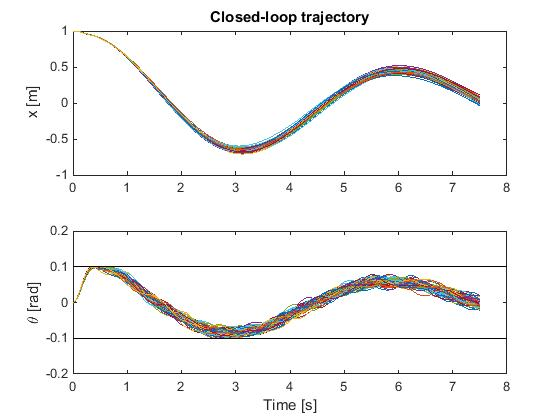
\includegraphics[width = 0.8\linewidth]{SCMPC_cartPenX.jpg}
		\label{fig:SCMPC_cartPenX}
	\end{subfigure}
	\begin{subfigure}{.45\textwidth}
		\centering
		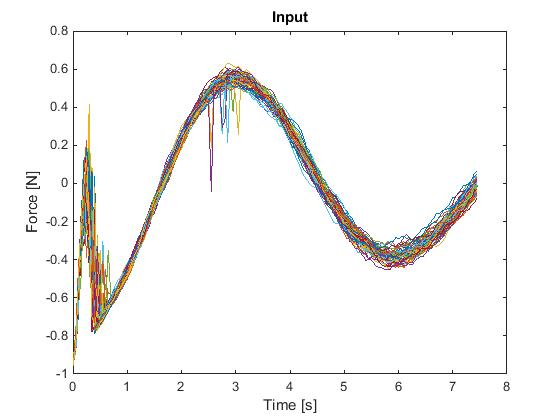
\includegraphics[width = 0.8\linewidth]{SCMPC_cartPenU.jpg}
		\label{fig:SCMPC_cartPenU}
	\end{subfigure}
	\caption{One the left, the cart position and pendulum angle are plotted for 50 simulations over 150 time steps. The applied control input is shown on the right.}
\end{figure}

The disturbance $w$ is a uniform scalar random variable so $\alpha = w^2$ has a density function given by $$ f_\alpha (x) = \begin{cases}
\frac{1}{2w_{max}\sqrt{x}} & 0 \leq x \leq w_{max}^2 \\
0 &	\mathrm{otherwise}
\end{cases} $$
This density function was used to find the tube scalings for the tube MPC implementation. To avoid evaluating $f_\alpha$ at zero, where it is infinite, a midpoint Riemann sum was used for numerical integration instead of the trapezoid rule.

\section{tables}

\begin{center}
\begin{tabular}{| r | c | c | c |}
	\hline
	& $V_{emp}^{(1)}$ & $V_{emp}^{(2)}$ & $\ell_{avg}$ \\ \hline
	AR & 0.20\% & 0.13\% & 9.49\\ \hline
	SCMPC & 9.87\%  & 10\% & 5.71 \\ \hline
	TMPC & 0.07\% & 0\% & 11.25\\ \hline
\end{tabular}
\end{center}

\begin{center}
	\begin{tabular}{| r | c | c |}
		\hline
		& $\bar{V}_{emp}$ & $C_{avg}$ \\ \hline
		AR    &        &  \\ \hline
		SCMPC & 8\%    &  \\ \hline
		TMPC  &        &  \\ \hline
	\end{tabular}
\end{center}


\bibliographystyle{plain}
\bibliography{sources}

\end{document}          
